\chapter{Zusammenfassung}
\section{Statistiken und Vergleiche der Pathfinding-Algorithmen}
\begin{center}
  \boxed{
    \textit{Alle notierten Messresultate pro Vergleich befinden sich im Anhang dieser Arbeit.}
  }
\end{center}

Das Autorenteam hat sich auf eine Rastergrösse von $50\times 50$ Felder
entschieden und durchlief die Vergleiche 125-mal. Die Rechenzeit wurde
auf 0.1ms gerundet. Die Diagonalen wurden mitbeachtet, da dies zu
Optimierten Strecken führen kann.

Diese 125 Versuche wurden zuerst in folgende Kategorien in den Resultate
unterteilt: Weg des kürzesten patinier von 0-10 Felder, 11-20 Felder,
21-30 Felder, 31-40 Felder, 41-50 Felder. Jede dieser Unterteilung hat
25 Vergleich Ergebnisse. Diese Unterteilung hat den Grund, dass auf
längeren Wege die Unterschiede nach der Erfahrung dieser Arbeit durch
das Autorenteam besser zu sehen sind.

\begin{longtable}[]{@{}l@{}}
\toprule
\endhead
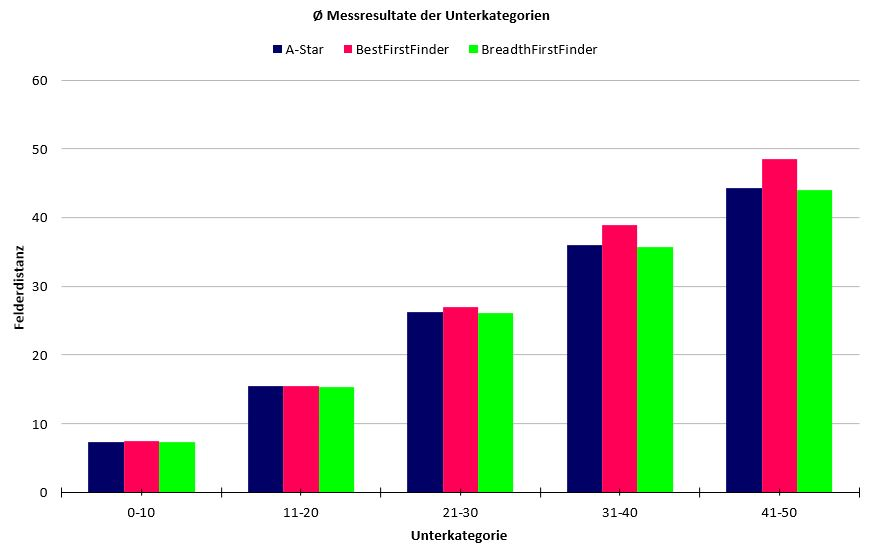
\includegraphics[width=6.26111in,height=4.02639in]{statistik_1.JPG}\tabularnewline
\bottomrule
\end{longtable}

Man erkennt gut, dass der A-Star und BreadthFirstFinder circa die gleiche
Felder Distanz Finden. Je Grösser der Abstand von Start und Ziel in
Feldern, desto grösser ist der Unterschied zwischen dem BestFirtFinder
und den anderen zwei.

\begin{longtable}[]{@{}l@{}}
\toprule
\endhead
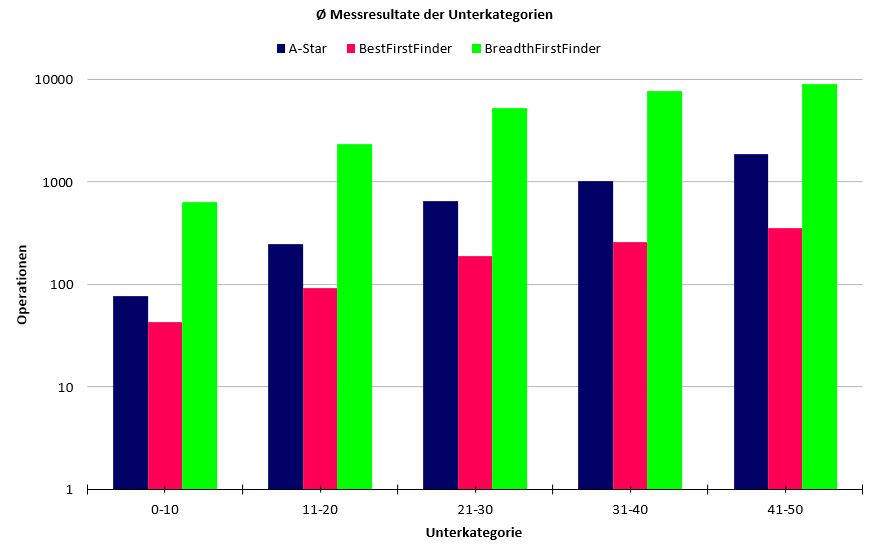
\includegraphics[width=6.26111in,height=3.95625in]{statistik_2.JPG}\tabularnewline
\bottomrule
\end{longtable}

Man beachte, die Diagramm-Darstellung ist Logarithmisch. Im Aufwand der
ausgeführten Operationen steigt der BreadthFirstFinder viel extremer als
die anderen. Der A-Star muss im Verhältnis zum BestFirstFinder immer
mehr Operationen Ausführen. Die Steigung des BreadthFirstFinder senkt
sich im Laufe der Felder Distanz, dies kommt daher, dass er am Rand des
Rasters ist und diese Seite nicht mehr weiter erkunden muss. Die
Vorteile einer Heuristik wird hier klar verdeutlicht, der A-Star und
BestFirstFinder müssen durch die Wahrscheinlichkeit Berechnung weniger
Operationen durchlaufen.

\begin{longtable}[]{@{}l@{}}
\toprule
\endhead
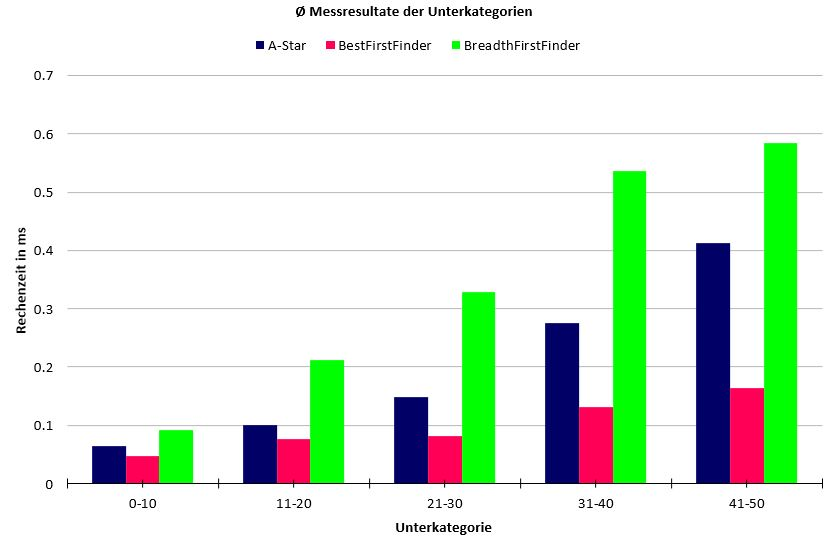
\includegraphics[width=6.26944in,height=4.15625in]{statistik_3.JPG}\tabularnewline
\bottomrule
\end{longtable}

Da der BestFirstFinder den erst besten Weg tiefer durchsucht, ist seine
Rechen Zeit um einiges verkürzt als die Anderen. Da der
BreadthFirstFinder am meisten Operationen hat, ist es logisch, dass
seine Rechen Zeit höher als A-Star oder BestFirstFinder ist.

\section{Interpretation Resultate}

Durch die Statistik Diagramme kann man folgendes herauslesen:

\begin{itemize}
\item
  Der A-Star und BreadthFirstFinder finden circa den gleich optimalen Weg,
  wobei der BreadthFirstFinder viel mehr an Operationen aufwenden muss,
  da er keine Heuristik besitzt.
\item
  Hat man begrenzte Zeit, so ist der BestFirstFinder gut geeignet, er
  findet nicht den Optimalsten Weg, spart dafür in Zeit und Operationen.
\item
  Je grösser das Raster, desto weniger ist der BreadthFirstFinder
  geeignet, da er zu viele Operationen benötigt und langsam wird im
  Vergleich zum A-Star.
\item
  Die Rechenzeit vom BestFirstFinder steigt linear, die Rechenzeit vom
  A-Star und BreadthFirstFinder exponential solange der
  BreadthFirstFinder keine Rasterseite erreicht hat.
\end{itemize}

